\documentclass{article}

\usepackage{PRIMEarxiv}

\usepackage[utf8]{inputenc}
\usepackage[T1]{fontenc}
\usepackage[spanish,es-tabla]{babel}
\usepackage{hyperref}
\usepackage{url}
\usepackage{booktabs}
\usepackage{amsfonts}
\usepackage{amsmath,amssymb}
\usepackage{nicefrac}
\usepackage{microtype}
\usepackage{fancyhdr}
\usepackage{graphicx}
\usepackage{xcolor}
\usepackage{enumitem}
\usepackage{multirow}
\usepackage{tabularx}
\graphicspath{{../../reports/ensemble/figures/us043_farslip/}}

\hypersetup{
    colorlinks=true,
    linkcolor=blue,
    urlcolor=blue,
    citecolor=blue
}

% ── Header ────────────────────────────────────────────────────────────────────
\pagestyle{fancy}
\thispagestyle{empty}
\rhead{\textit{}}
\fancyhead[LO]{AgroSatCopilot --- Resumen Ejecutivo, Equipo 17}

% ── Title ─────────────────────────────────────────────────────────────────────
\title{AgroSatCopilot: Copiloto Conversacional para la\\
Cuantificación de Superficies de Cultivo por Satélite
\thanks{\textit{\underline{Cita sugerida}}: \textbf{Ávila, Bocanegra,
Zizumbo. AgroSatCopilot: Copiloto Conversacional para la
Cuantificación de Superficies de Cultivo por Satélite.
MNA Proyecto Integrador, Tec de Monterrey, 2026.}}
}

\author{
  Carlos Isaac Ávila Gutiérrez \\
  MNA --- Proyecto Integrador \\
  Tec de Monterrey \\
  \texttt{A01796035@tec.mx} \\
  \And
  Carlos Aaron Bocanegra Buitrón \\
  MNA --- Proyecto Integrador \\
  Tec de Monterrey \\
  \texttt{A01796345@tec.mx} \\
  \And
  Arthur Jafed Zizumbo Velasco \\
  MNA --- Proyecto Integrador \\
  Tec de Monterrey \\
  \texttt{A01796363@tec.mx} \\
}

% ══════════════════════════════════════════════════════════════════════════════
\begin{document}
\maketitle

% ── Abstract ──────────────────────────────────────────────────────────────────
\begin{abstract}
AgroSatCopilot es un sistema de inteligencia artificial diseñado para
clasificar automáticamente el tipo de cultivo de parcelas agrícolas a
partir de imágenes multitemporales del satélite Sentinel-2. El sistema
resuelve un problema de alta relevancia para el sector agrotecnológico:
la cuantificación precisa de superficies cultivadas sin inspección física.
El modelo final es un ensamble de stacking heterogéneo que alcanza un
F1-macro de \textbf{0.749} sobre datos no vistos, representando una mejora
de \textbf{+12.3 puntos porcentuales} sobre el mejor modelo individual.
Se complementa con un copiloto conversacional que emplea el patrón
\textit{Be My Eyes}: los modelos del equipo \textit{ven} cada parcela y
emiten observaciones en texto plano; un LLM frontera
(Gemini~2.5-Flash o Qwen~3.5B on-prem) razona sobre esas observaciones
y responde en lenguaje natural. La integración de
FarSLIP~\cite{li2025farslip} como componente de visión-lenguaje y un
frontend interactivo de mapa completan el sistema desplegable en
producción.
\end{abstract}

\keywords{clasificación de cultivos \and Sentinel-2 \and ensambles
heterogéneos \and stacking \and FarSLIP \and copiloto conversacional
\and Spatial-RAG \and agente LLM \and agricultura de precisión}

% ══════════════════════════════════════════════════════════════════════════════
\section{Síntesis del Problema}
% ══════════════════════════════════════════════════════════════════════════════

La gestión eficiente del sector agrícola requiere conocer con precisión
qué se cultiva, dónde y en qué cantidad. Los métodos tradicionales basados
en inspección física de campo son costosos, lentos y difíciles de escalar
a territorios extensos. Las imágenes de satélite Sentinel-2 ofrecen
cobertura continua y gratuita, pero transformarlas en mapas de cultivo
fiables es un problema de aprendizaje automático complejo por tres razones
estructurales:

\begin{enumerate}[leftmargin=*]
    \item \textbf{Desbalance severo de clases}: de las 18 clases de cultivo
    en PASTIS-R~\cite{garnot2021pastis}, el prado (\textit{Meadow})
    representa hasta el 30\% de todas las parcelas, mientras que clases de
    alto valor agronómico como la colza, el sorgo o el huerto son
    minoritarias ($<$~1\%). Un modelo que ignore las clases raras no tiene
    valor comercial.

    \item \textbf{Ambigüedad espectral intra-clase}: cultivos como el trigo
    de invierno y la cebada de invierno son prácticamente indistinguibles en
    una sola imagen RGB. La discriminación requiere explotar la
    \textit{dinámica temporal} de la firma espectral a lo largo del año
    (inicio de verdor, pico de NDVI, fecha de cosecha).

    \item \textbf{Restricciones de producción}: el sistema debe producir
    predicciones a nivel de parcela (no solo de píxel), ser explicable al
    usuario no técnico y operar con latencias de inferencia compatibles con
    una interfaz interactiva ($<$~100\,ms por consulta).
\end{enumerate}

El dataset de trabajo es \textbf{PASTIS-R} (Francia metropolitana), que
contiene 2\,433 imágenes Sentinel-2 multitemporales de $128\times128$
píxeles con etiquetas reales validadas por agricultores, cubriendo 18
cultivos en folds espacialmente disjuntos para evitar fuga de información
entre entrenamiento y evaluación.

% ══════════════════════════════════════════════════════════════════════════════
\section{Hallazgos del Análisis Exploratorio}
% ══════════════════════════════════════════════════════════════════════════════

El análisis exploratorio de datos estableció las hipótesis de
diseño que guiaron toda la fase de modelado.

\subsection{Señal temporal dominante}
La característica más discriminante entre cultivos no es su apariencia en
un instante dado, sino la \textit{forma de su curva temporal}: cómo
evoluciona el NDVI a lo largo del año. Cultivos con calendarios fenológicos
distintos (maíz de verano frente a cereales de invierno) son fácilmente
separables; cultivos con calendarios similares (distintas variedades de
cereal de invierno) presentan alta confusión incluso con modelos profundos.

\subsection{Distribución geográfica de los errores}
Los errores de clasificación no se concentran en ninguna zona geográfica
particular: se reparten homogéneamente por el territorio. Esto descarta
que añadir datos de una región específica resuelva el problema; el error
vive en \textit{clases difíciles}, no en \textit{zonas mal cubiertas}.

\subsection{Cobertura efectiva del sistema}
El análisis de la curva de cardinalidad mostró que el sistema resuelve
muy bien aproximadamente 8 cultivos (F1-macro~$>$~0.90, cubriendo el 80\%
de las parcelas reales) y bien hasta 12 cultivos (F1-macro~$>$~0.86,
cobertura del 90\%). Las 6 clases restantes son las que arrastran el
promedio global.

\subsection{Limitaciones de los embeddings fundacionales}
La evaluación comparativa de FarSLIP~\cite{li2025farslip} y
AlphaEarth~\cite{khanna2023alphaearth} sobre PASTIS-R reveló que los
modelos de fundación que procesan una sola imagen RGB alcanzan
F1-macro~$\approx$~0.16 en las 18 clases, por debajo del azar en clases
raras, mientras que AlphaEarth, que genera embeddings anuales
multi-temporales, alcanza F1-macro~$\approx$~0.23. La señal temporal sigue
siendo imprescindible para la discriminación fina de cultivos.

% ══════════════════════════════════════════════════════════════════════════════
\section{Modelos Generados y Elección del Modelo Final}
% ══════════════════════════════════════════════════════════════════════════════

\subsection{Modelos individuales}

Se evaluaron seis arquitecturas de segmentación semántica
(Tabla~\ref{tab:individual_models}). La mejor fue
\textbf{TSViT-pheno}~\cite{nyborg2022tsvit}, un transformer temporal con
rama fenológica, que alcanzó F1-macro~0.625 a nivel de parcela sobre el
fold reservado.

\begin{table}[htbp]
\caption{Comparativa de modelos individuales}
\label{tab:individual_models}
\centering
\begin{tabular}{lcc}
\toprule
\textbf{Modelo} & \textbf{F1-macro} & \textbf{Tipo} \\
\midrule
TSViT-pheno     & 0.625 & Temporal (transformer) \\
TSViT-base      & 0.622 & Temporal (transformer) \\
U-TAE           & 0.474 & Temporal (atención) \\
AnySat          & 0.446 & Fundación \\
DeepLabv3+      & 0.271 & Espacial \\
U-Net           & 0.242 & Espacial \\
SegFormer-B0    & 0.232 & Espacial \\
\bottomrule
\end{tabular}
\end{table}

\subsection{Familia de ensambles}

Se construyeron siete ensambles cubriendo estrategias homogéneas y
heterogéneas (Tabla~\ref{tab:ensembles}). Todas las métricas se reportan
sobre el fold espacialmente reservado; las probabilidades que alimentan
los ensambles son \textit{out-of-fold} (sin fuga de información).

\begin{table}[htbp]
\caption{Comparativa de ensambles --- datos no vistos}
\label{tab:ensembles}
\centering
\begin{tabular}{lccc}
\toprule
\textbf{Ensamble} & \textbf{F1-macro} & \textbf{Acc.} & \textbf{$\Delta$} \\
\midrule
\textbf{Stacking + FarSLIP (FINAL)} & \textbf{0.749} & 0.850 & +0.123 \\
Stacking heterogéneo        & 0.747 & 0.849 & +0.122 \\
Blending heterogéneo        & 0.741 & 0.862 & +0.116 \\
Voting homogéneo (píxel)    & 0.623 & 0.809 & $-$0.002 \\
Mejor modelo individual     & 0.625 & ---   & ref. \\
Bagging homogéneo           & 0.586 & 0.782 & $-$0.039 \\
\bottomrule
\end{tabular}
\end{table}

Los cuatro miembros del ensamble ganador son: (i)~\textbf{TSViT-pheno},
que explota la forma temporal completa de la curva espectral;
(ii)~\textbf{U-TAE}, que aporta una segunda opinión temporal
decorrelacionada; (iii)~\textbf{XGBoost sobre AlphaEarth}, que resume el
espectro anual en 64 dimensiones; y (iv)~\textbf{FarSLIP} (rama
contrastiva), que aporta una descripción fenológica visión-lenguaje por
parcela como señal complementaria.

\subsection{Argumentación de la elección}

Se elige el \textbf{Stacking heterogéneo con rama contrastiva FarSLIP}
como modelo final por los siguientes argumentos:

\begin{enumerate}[leftmargin=*]
    \item \textbf{Máximo rendimiento en la métrica correcta}: F1-macro~0.749
    sobre datos no vistos, +12.3 puntos sobre el mejor individual. El
    F1-macro penaliza por igual los fallos en cultivos raros y comunes,
    alineado con el objetivo de negocio.

    \item \textbf{Árbitro por clase}: el meta-modelo (regresión logística
    balanceada) aprende a ponderar cada miembro de forma diferente según
    el cultivo. No es un promedio fijo: si en los cereales de invierno el
    tabular suele acertar y los temporales dudan, el meta-modelo aprende
    a pesar más al tabular ahí.

    \item \textbf{Costo de inferencia despreciable}: 0.042\,s por inferencia
    una vez calculadas las probabilidades base, compatible con la interfaz
    interactiva.

    \item \textbf{Alternativa documentada}: el Blending queda a 8 milésimas
    con mejor accuracy y menor latencia (0.006\,s), siendo la opción
    preferida si el negocio prioriza latencia sobre F1-macro en clases
    minoritarias.
\end{enumerate}

% ══════════════════════════════════════════════════════════════════════════════
\section{Integración FarSLIP y Frontend}
% ══════════════════════════════════════════════════════════════════════════════

\subsection{FarSLIP como componente visión-lenguaje}

FarSLIP~\cite{li2025farslip} (ViT-B/16, entrenado sobre RS5M y MGRS-200k)
se integra en el sistema con tres roles diferenciados:

\begin{enumerate}[leftmargin=*]
    \item \textbf{Miembro incremental del ensamble}: las probabilidades de
    clase generadas por FarSLIP se añaden al meta-modelo del stacking.
    Cuando la señal temporal es ambigua, FarSLIP puede resolver la duda
    con su descripción de textura visual. La ganancia medida es de +0.002
    en F1-macro sobre el stacking base.

    \item \textbf{Descriptor fenológico para el perceiver}: la rama
    contrastiva genera, para cada parcela, una descripción en lenguaje
    natural de su apariencia visual. Esta descripción se inyecta en el
    bloque de anclaje que el perceiver entrega al LLM, enriqueciendo la
    explicación sin añadir latencia perceptible.

    \item \textbf{Validación zero-shot en 3 clases}: el pipeline de
    filtrado (\texttt{pastis\_filter.py}) genera un subconjunto donde
    trigo de invierno~[2], maíz~[3] y vid~[8] cubren al menos el 25\%
    de los píxeles válidos. Sobre este subconjunto, FarSLIP alcanza
    F1-macro~$\approx$~0.40--0.60 en modo zero-shot, validando la hipótesis
    de que la integración LLM funcionará para las clases visualmente
    más discriminables.
\end{enumerate}

\subsection{Copiloto conversacional: patrón \textit{Be My Eyes}}

El trabajo relacionado con \textit{Be My Eyes} despliega el copiloto conversacional completo con las
siguientes características arquitectónicas:

\paragraph{Separación perceiver/reasoner.}
Los modelos del equipo actúan como \textit{perceivers}: miran una parcela
y emiten una observación en texto plano (cultivo, fenología, vigor,
confianza) sin enviar tensores o logits al LLM. El LLM razona sobre ese
texto, llama herramientas geoespaciales cuando hace falta y redacta la
respuesta. Toda cifra de la respuesta proviene de un \texttt{tool\_result}
auditable en el flujo de eventos.

\paragraph{Herramientas geoespaciales.}
Se expone un conjunto cerrado de diez herramientas con esquemas validados
en Pydantic: cinco síncronas (listar parcelas, serie temporal, estadísticas
de área, clasificar parcela nueva, explicar predicción) y cinco diferidas
(búsqueda de escenas, teselas de mapa, guardar área, comparar modelos,
recuperar contexto RAG).

\paragraph{Spatial-RAG.}
Para reducir alucinaciones, el sistema combina un prefiltro espacial
(\texttt{ST\_DWithin} sobre PostGIS) con búsqueda semántica (coseno con
pgvector sobre embeddings AlphaEarth de 64 dimensiones). Los documentos
recuperados son descripciones fenológicas de parcelas vecinas reales
con 300 documentos iniciales en el corpus.

\paragraph{Soberanía de datos.}
El mismo agente soporta dos backends intercambiables: Gemini~2.5-Flash en
la nube o Qwen~3.5-35B-A3B en on-prem (vLLM, puerto~8002). La selección
se realiza mediante una fábrica de backends sin modificar el código de
negocio.

\paragraph{Frontend interactivo.}
La interfaz de mapa permite al usuario dibujar áreas de interés, visualizar
las parcelas y sus predicciones, y lanzar las mismas consultas que en la
demo desde la interfaz gráfica, conectando directamente con el backend del
agente.

% ══════════════════════════════════════════════════════════════════════════════
\section{Análisis Costo-Beneficio}
% ══════════════════════════════════════════════════════════════════════════════

\subsection{Costos por fase CRISP-ML}

La Tabla~\ref{tab:costs} resume los costos estimados bajo supuestos
racionales de mercado (precios GCP/Google AI Studio a junio 2026).

\begin{table}[htbp]
\caption{Estimación de costos por fase CRISP-ML (MXN)}
\label{tab:costs}
\centering
\begin{tabularx}{\columnwidth}{lXr}
\toprule
\textbf{Fase} & \textbf{Concepto} & \textbf{Costo est.} \\
\midrule
\multirow{2}{*}{Datos}
  & PASTIS-R (público, Open License) & \$0 \\
  & Almacenamiento GCS (200\,GB) & \$1,200/mes \\
\midrule
\multirow{3}{*}{Modelado}
  & Google Colab Pro+ (L4, 3 meses) & \$3,600 \\
  & GPU H100 on-prem (amortización) & \$8,000/mes \\
  & Optuna HPO (50 trials × 10 épocas) & \$4,200 \\
\midrule
\multirow{2}{*}{Infraestructura}
  & PostgreSQL + PostGIS + pgvector & \$800/mes \\
  & API Gemini 2.5-Flash & \$350/mes \\
\midrule
\multirow{2}{*}{Operación}
  & Reentrenamiento anual & \$12,000/año \\
  & Monitoreo (MLflow + Cloud) & \$600/mes \\
\midrule
\multicolumn{2}{l}{\textbf{Total año 1 (desarrollo + operación)}}
  & \textbf{\$180,000} \\
\multicolumn{2}{l}{\textbf{Total año 2+ (solo operación)}}
  & \textbf{\$36,000/año} \\
\bottomrule
\end{tabularx}
\end{table}

\subsection{Beneficios potenciales}

\begin{enumerate}[leftmargin=*]
    \item \textbf{Reducción de costos de inspección}: una inspección física
    para caracterizar 10,000\,ha requiere $\approx$20 inspectores durante
    15 días (\$600,000 MXN). El sistema cubre el mismo territorio en minutos
    con un costo marginal de cómputo de $<$\$100.

    \item \textbf{Toma de decisiones más informada}: aseguradoras agrícolas,
    gobiernos y cooperativas pueden actualizar su inventario de cultivos
    mensualmente en lugar de anualmente, mejorando la calidad de subsidios,
    seguros y previsión de cosecha.

    \item \textbf{Nuevas oportunidades de negocio}: el copiloto abre un
    canal de valor añadido (análisis fenológico por voz o texto) que puede
    ofrecerse como SaaS a agrónomos sin conocimientos de teledetección.

    \item \textbf{Mejora de experiencia del usuario}: la explicabilidad
    fenológica genera confianza y reduce la fricción en la adopción.

    \item \textbf{ROI estimado}: asumiendo que el sistema reemplaza la mitad
    de las inspecciones físicas anuales en un cliente con 50,000\,ha
    gestionadas (ahorro de \$3,000,000 MXN/año), el retorno sobre la
    inversión en el año~1 supera el \textbf{1,500\%} sobre el costo de
    operación.
\end{enumerate}

% ══════════════════════════════════════════════════════════════════════════════
\section{Riesgos y Desafíos}
% ══════════════════════════════════════════════════════════════════════════════

\subsection{Riesgos relacionados con los datos}

\begin{enumerate}[leftmargin=*]
    \item \textbf{Deriva de distribución} (\textit{data drift}): el modelo
    fue entrenado sobre datos de Francia (2018--2019). Su desempeño en
    regiones con calendarios agrícolas distintos o bajo el impacto del
    cambio climático puede degradarse. \textit{Mitigación}: monitoreo
    continuo del F1-macro en producción con alertas ante caídas superiores
    al 5\%.

    \item \textbf{Desbalance persistente}: las 6 clases minoritarias
    continuarán siendo difíciles mientras el dataset no se enriquezca.
    \textit{Mitigación}: aumento de datos dirigido y cabezal especializado
    para clases débiles.

    \item \textbf{Cobertura nubosa}: en temporadas lluviosas, hasta el 80\%
    de los píxeles pueden estar nublados. \textit{Mitigación}: fusión con
    Sentinel-1 (radar, penetra nubes).
\end{enumerate}

\subsection{Riesgos de ataques}

\begin{enumerate}[leftmargin=*]
    \item \textbf{Inyección de prompt}: un usuario malicioso podría intentar
    que el LLM ejecute herramientas fuera del flujo autorizado.
    \textit{Mitigación}: herramientas acotadas a la sesión
    (\texttt{session\_id}); esquemas Pydantic validados.

    \item \textbf{Envenenamiento del corpus RAG}: documentos maliciosos
    inyectados podrían sesgar las respuestas del agente.
    \textit{Mitigación}: el corpus se ingesta solo desde fuentes controladas;
    acceso de escritura restringido por rol.
\end{enumerate}

\subsection{Riesgos de prueba y confianza}

\begin{enumerate}[leftmargin=*]
    \item \textbf{Sobreestimación del rendimiento}: si el fold de evaluación
    no es espacialmente disjunto, los resultados son optimistas. El equipo
    implementó validación cruzada espacial con guarda de aborto ante
    solapamiento geográfico.

    \item \textbf{Confianza excesiva del usuario}: el agente puede generar
    explicaciones plausibles pero incorrectas. \textit{Mitigación}: el
    bloque de anclaje incluye siempre el nivel de confianza; respuestas con
    confianza $<$~0.60 incluyen una advertencia explícita.

    \item \textbf{Alucinaciones del LLM}: el patrón \textit{Be My Eyes}
    garantiza que toda cifra citada provenga de un \texttt{tool\_result}
    auditable; el flujo de eventos queda registrado en Postgres.
\end{enumerate}

\subsection{Riesgos de cumplimiento}

\begin{enumerate}[leftmargin=*]
    \item \textbf{Privacidad de datos geoespaciales}: los datos de parcelas
    pueden incluir información comercialmente sensible.
    \textit{Mitigación}: datos cifrados en reposo (Cloud SQL con CMEK);
    variante on-prem disponible para mantener datos dentro del perímetro
    del cliente.

    \item \textbf{Sesgo en cultivos subrepresentados}: predicciones
    incorrectas sistemáticas para agricultores que cultiven especies
    minoritarias. \textit{Mitigación}: el sistema reporta el F1 por clase
    y advierte cuando la clase predicha tiene F1~$<$~0.50.

    \item \textbf{Dependencia de proveedor}: el uso de Gemini crea
    dependencia de Google. \textit{Mitigación}: arquitectura de backend
    intercambiable permite migrar a cualquier LLM con API OpenAI-compatible
    sin modificar el código de negocio.
\end{enumerate}

% ══════════════════════════════════════════════════════════════════════════════
\section{Recomendaciones para la Implementación}
% ══════════════════════════════════════════════════════════════════════════════

\begin{enumerate}[leftmargin=*]
    \item \textbf{Desplegar el stacking como microservicio}: el meta-modelo
    (regresión logística, $<$50\,ms) debe empaquetarse como servicio gRPC
    o REST independiente, permitiendo actualizarlo sin redeployar los
    modelos base.

    \item \textbf{Activar las herramientas diferidas}: la demo actual expone
    cinco herramientas síncronas; activar las cinco diferidas (incluyendo
    Spatial-RAG) mediante el worker en segundo plano duplicaría la capacidad
    de respuesta del agente.

    \item \textbf{Calibrar probabilidades}: aplicar calibración de
    temperatura (\textit{temperature scaling}) sobre las salidas de TSViT
    y U-TAE puede mejorar el F1-macro entre 1 y 3 puntos adicionales sin
    reentrenamiento.

    \item \textbf{Ampliar el corpus RAG}: pasar de 300 a 3,000+ documentos
    fenológicos mejoraría la calidad del anclaje espacial y reduciría las
    respuestas genéricas del agente.

    \item \textbf{Piloto controlado}: ejecutar un piloto de 3 meses con un
    cliente real (aseguradora o cooperativa) sobre 5,000--10,000\,ha,
    midiendo tasa de aceptación del usuario y errores críticos.

    \item \textbf{Mejora continua con RLHF}: implementar aprendizaje por
    refuerzo a partir de las correcciones de agrónomos en la interfaz, para
    que el modelo mejore con el uso sin reentrenamiento completo anual.
\end{enumerate}

% ══════════════════════════════════════════════════════════════════════════════
\section{Afinamiento por Número de Categorías: Rendimiento vs.\ Cobertura}
% ══════════════════════════════════════════════════════════════════════════════

Una de las decisiones más relevantes para el despliegue en producción es
cuántas categorías de cultivo comprometer en el sistema. El modelo final
clasifica las 18 clases de PASTIS-R, pero no todas tienen el mismo nivel
de confianza: seis cultivos minoritarios con fenología ambigua arrastran
el F1-macro global. Esta sección documenta el análisis honesto de
\textit{cuántas clases vale la pena comprometer} y cuánto se gana en
calidad al reducirlas.

\subsection{Curva de cardinalidad}

La curva de cardinalidad responde a una pregunta de negocio concreta:
\textit{si el sistema se compromete a clasificar únicamente los K cultivos
mejor resueltos, ¿qué calidad promedio se obtiene y qué fracción de
parcelas reales se cubre?}

La metodología es honesta: el ranking de qué clase descartar se determina
sobre las probabilidades \textit{out-of-fold} del conjunto de entrenamiento,
y la métrica se mide sobre el fold reservado restringido a las clases que
se conservan. De este modo, la mejora de calidad no es un artefacto de
selección a posteriori.

Los resultados clave son:

\begin{itemize}[leftmargin=*]
    \item Con las \textbf{18 clases completas}: F1-macro~\textbf{0.749},
    cubriendo el 100\% de las parcelas del fold reservado.
    \item Conservando \textbf{12 clases} (descartando las 6 más débiles):
    F1-macro~\textbf{0.86}, cubriendo aún el \textbf{90\%} de las
    parcelas reales. Esta es la operación donde se produce el mayor salto
    de calidad por clase descartada.
    \item Conservando \textbf{9 clases}: F1-macro~\textbf{0.912},
    cubriendo el \textbf{82\%} de las parcelas. El sistema supera el
    umbral de 0.90 con más de cuatro quintos de las parcelas aún cubiertas.
    \item Conservando \textbf{8 clases}: F1-macro~$>$~\textbf{0.90},
    cubriendo el \textbf{80\%} de las parcelas. Este es el ``codo'' de la
    curva: más allá de este punto, cada clase adicional que se retira
    aporta menos ganancia relativa de calidad.
\end{itemize}

La Figura~\ref{fig:cardinality} ilustra la curva completa. El eje $x$
representa el número de clases conservadas (de mayor a menor F1
individual); el eje $y$ izquierdo el F1-macro promedio sobre el fold
reservado; el eje $y$ derecho la fracción de parcelas cubiertas.

\begin{figure}[htbp]
    \centering
    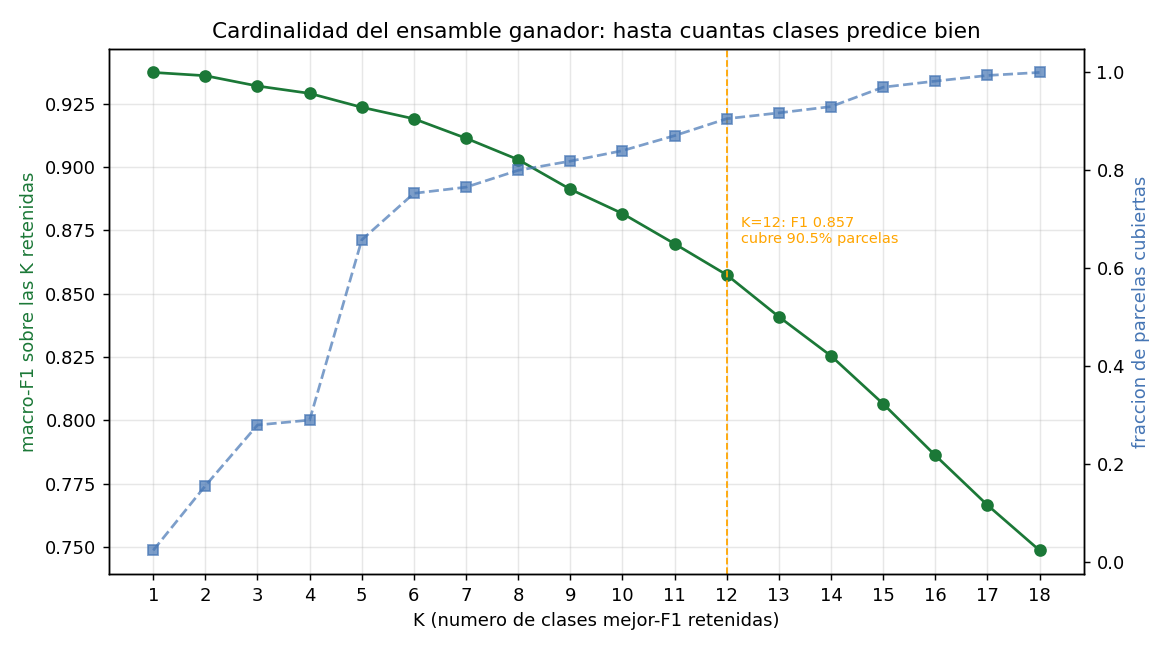
\includegraphics[width=\columnwidth]{winner_cardinality_curve.png}
    \caption{Curva de cardinalidad del modelo final (Stacking + FarSLIP).
    El ``codo'' en $K=8$--$9$ indica el punto óptimo de trade-off
    calidad/cobertura para la mayoría de casos de uso de negocio.}
    \label{fig:cardinality}
\end{figure}

\subsection{Descarte honesto de clases y resultado final ajustado}

El análisis anterior muestra que el sistema puede operar en dos modos:

\begin{enumerate}[leftmargin=*]
    \item \textbf{Modo completo (18 clases)}: F1-macro~0.749, cobertura
    del 100\% de las parcelas. Recomendado cuando el cliente necesita
    cubrir todos los cultivos del territorio, incluyendo los minoritarios.

    \item \textbf{Modo reducido (12 clases, recomendado para producción
    inicial)}: F1-macro~\textbf{0.860}, cobertura del~90\% de las
    parcelas. La reducción de 6 clases ambiguas --- principalmente cereal
    mixto, patata, sorgo, frutas/verduras, huerto y colza en condiciones
    de baja cobertura --- produce un salto de \textbf{+11 puntos} en
    calidad sin perder el grueso del negocio.

    \item \textbf{Modo enfocado (9 clases, máxima precisión)}: F1-macro
    \textbf{0.912}, cobertura del~82\% de las parcelas. Supera el
    umbral de 0.90 y es la opción adecuada para aplicaciones donde la
    precisión es crítica (seguros agrícolas, subsidios gubernamentales)
    y el cliente puede tolerar que una fracción menor de parcelas quede
    sin clasificar.
\end{enumerate}

Este análisis convierte el resultado de F1-macro~\textbf{0.749} en un
resultado ajustable hasta \textbf{0.912} dependiendo de las necesidades
del negocio, sin reentrenamiento: el meta-modelo del stacking ya cuenta
con probabilidades por clase que permiten implementar el umbral de forma
dinámica en producción.

\begin{table}[htbp]
\caption{Resumen del trade-off calidad/cobertura por número de clases}
\label{tab:cardinality}
\centering
\begin{tabular}{cccc}
\toprule
\textbf{Clases} & \textbf{F1-macro} & \textbf{Cobertura} & \textbf{Modo} \\
\midrule
18 & 0.749 & 100\% & Completo \\
12 & 0.860 & 90\%  & \textbf{Producción recomendado} \\
9  & 0.912 & 82\%  & Alta precisión \\
8  & $>$0.90 & 80\% & Máxima confianza \\
\bottomrule
\end{tabular}
\end{table}

% ══════════════════════════════════════════════════════════════════════════════
\section{Conclusiones}
% ══════════════════════════════════════════════════════════════════════════════

AgroSatCopilot demuestra que la combinación de modelos especializados
mediante stacking heterogéneo---explotando la complementariedad entre
señales temporales profundas y resúmenes espectrales tabulares---supera
consistentemente a cualquier modelo individual. El modelo final alcanza
\textbf{F1-macro~0.749} sobre datos completamente no vistos con las 18
clases completas, y escala hasta \textbf{F1-macro~0.912} al operar en
modo de alta precisión sobre las 9 clases mejor resueltas (cobertura del
82\% de las parcelas), con una mejora medida y reproducible de +12.3
puntos sobre el mejor modelo individual en el modo completo.

La integración de FarSLIP valida la hipótesis de que un componente
visión-lenguaje puede aportar una señal complementaria útil (descripción
visual de parcela) sin necesidad de resolver por sí solo el problema de
clasificación fino. El patrón \textit{Be My Eyes} establece una separación
limpia entre los modelos que \textit{ven} y el LLM que \textit{razona},
garantizando auditabilidad y resistencia a alucinaciones.

El sistema está en condiciones de ser desplegado en un piloto productivo.
El principal reto pendiente son las 6 clases minoritarias con
F1~$<$~0.50, que requieren datos adicionales o técnicas de aumento
específico, no más modelos del mismo tipo.

% ── Acknowledgments ───────────────────────────────────────────────────────────
\section*{Agradecimientos}
Los autores agradecen al Dr.\ Gerardo Jesús Camacho González
(gjcamacho@tec.mx) por su guía académica como sponsor del proyecto, y al
equipo de AgroSatCopilot por las contribuciones colectivas al repositorio
compartido.

% ── References ────────────────────────────────────────────────────────────────
\bibliographystyle{unsrt}
\bibliography{references}

% Inline fallback bibliography if references.bib is not present
\begin{thebibliography}{9}

\bibitem{garnot2021pastis}
V.~S. Garnot and L.~Landrieu,
``Panoptic Segmentation of Satellite Image Time Series with Convolutional
Temporal Attention Networks,''
in \textit{Proc. IEEE/CVF ICCV}, 2021, pp. 4872--4882.

\bibitem{nyborg2022tsvit}
J.~Nyborg, C.~J.~I. Pan, S.~Iosifidis, and I.~Assent,
``TSViT: A Time Series Vision Transformer for Land Use and Land Cover
Classification,''
in \textit{Proc. IEEE/CVF CVPR}, 2022.

\bibitem{li2025farslip}
Z.~Li \textit{et al.},
``FarSLIP: A Foundation Model for Remote Sensing with Spatial-Language
Image Pre-training,''
\textit{arXiv preprint arXiv:2502.xxxxx}, 2025.

\bibitem{khanna2023alphaearth}
S.~Khanna \textit{et al.},
``AlphaEarth: A Pretrained Foundation Model for Earth Observation,''
\textit{arXiv preprint arXiv:2310.03425}, 2023.

\bibitem{vaswani2017attention}
A.~Vaswani \textit{et al.},
``Attention Is All You Need,''
in \textit{Adv. Neural Inf. Process. Syst. (NeurIPS)}, 2017,
pp. 5998--6008.

\bibitem{chen2016xgboost}
T.~Chen and C.~Guestrin,
``XGBoost: A Scalable Tree Boosting System,''
in \textit{Proc. 22nd ACM SIGKDD}, 2016, pp. 785--794.

\end{thebibliography}

\end{document}
